\documentclass[aps, jcp, prb, two column, showpacs,groupedaddress,]{revtex4-2}
\usepackage{amsfonts,amsmath,amssymb}
\usepackage[none]{hyphenat}
\usepackage{fancyhdr}
\usepackage{graphicx}
\usepackage{hyperref}
\usepackage{float}
\usepackage{subfigure}
\usepackage{dcolumn}
\usepackage{multirow}
\usepackage{bm} 
\usepackage{lipsum}
\usepackage{gensymb}  
\hyphenation{ALPGEN}
\hyphenation{EVTGEN}
\hyphenation{PYTHIA}
%\topmargin 0.5cm
\usepackage[left= 1 in, right= 1 in, top= 0.5 in , bottom= 1 in]{geometry}
\parskip 0.2cm
\usepackage{hyperref}
\usepackage{xcolor} 
\hypersetup{ colorlinks, citecolor=blue ,linkcolor=black }


\usepackage{chemfig}

\newcommand{\abbrlabel}[1]{\makebox[3.5cm][l]{ {#1} }}
\newenvironment{abbreviations}{\begin{list}{}{\renewcommand{\makelabel}{\abbrlabel}}}{\end{list}}
\usepackage{hyperref}
\hypersetup{linktocpage}

\newcommand{\blue}[1]{\textcolor{blue}{#1}}
\title{bibliography}
\fancyhead{}
\fancyfoot{}
\fancyfoot[C]{\thepage}
\renewcommand{\footrulewidth}{0pt}


\begin{document}
	\vspace*{0.35in}

	
    \title{A STUDY OF CASEIN CONTENT IN DIFFERENT MILK SAMPLES OF LUMBINI DAIRY MILK}
	
	
	\author{Aaditya Prasad Gupta$^{1}$}	
	
	\affiliation{$^{1}$Tilottama Campus, Yogikuti, Rupandehi, Nepal.\\
	aadityaprasad.gupta@gmail.com}

	\begin{abstract}
			\addcontentsline{toc}{chapter}{Abstract} \noindent  This study examines the amount of casein present in different sample of milk and comparison between the protein found in those sample. 
\\

		
	\end{abstract}
	
	\maketitle
\tableofcontents
%\newpage

\section{Introduction}

Natural milk is an opaque white fluid secreted by the mammary glands of female mammals.The main constituents of natural milk are protein, carbohydrate, minerals, vitamins, fats and qatar are considered as a complete balanced diet. Fresh milk is sweetish in taste. However, when it is kept for a long time at a temperature of $5^{0}$C, it becomes sour because of bacteria present in the air. These bacteria convert lactose of milk into sour lactic acid. In acidic conditions, the casein of milk starts separating as a precipitate. When the acidity in milk is sufficient and the temperature is around $36^{0}$C it forms a semi-solid mass, called curd. Cow's milk contains about 3\%. Casein is a family of related phospho-proteins. Casein is present in milk as calcium caseinate in the form of micelles. These micelles have a negative charge and on adding acid to milk the negative charges are neutralized.

Calcium caseinate + acetic acid \rightarrow casein$_{(s)}$+ calcium acetate$_{(aq)}$

Milk also contains Casein, the chief protein in milk and the essential ingredient of cheese. In pure form, it is an amorphous white solid, tasteless and odorless, while its commercial type is yellowish with a pleasing odor. Dry casein keeps well if protected from insects and rodents: damp casein is quickly attacked by molds and bacteria and acquires a disagreeable odour. The specific gravity is 1.25 to 1.31

Casein is a mixture of phosphoproteins of differing molecular weight. Casein is usually made from skim milk (rarely from buttermilk), by one of three methods:

\begin{enumerate}
    \item Naturally soured casein curdles when enough lactic acid develops from fermentation of milk sugar by the ever present bacterium streptococcus lactis. \vspace{-0.1cm}
    \item Acid casein is precipitated by adding dilute hydro-chloric acid or sulphuric acid. \vspace{-0.1cm}
    \item For rennet casein, warm skim milk is set with rennet extract until the calcium paracaseinate clots, after which the clot is cut into small pieces to allow the whey to drain. In all three methods the whey is drawn off, the curd washed with water, drained or pressed, dried in warm air, ground, and packed for sale. Rennet casein retains much of the calcium phosphate from the milk. \vspace{-0.1cm}
\end{enumerate}


Casein is used in prepared foods, in medicines and dietary supplements, and in cosmetics. Minor industrial applications include the seasoning and dressing of leather, cleaners and polishes for shoes, textiles printing and sizing, insecticides sprays, soap making and many uses in which casein serves as a protective colloid, emulsifying agent or binder. Major applications of caseins are paper coatings, glues, paint, plastics and man made fibres.


\section{Requirements}

\begin{enumerate}
    \item Beakers(250 ml) \vspace{-0.1cm}
    \item Filtration flasks \vspace{-0.1cm}
    \item Measuring cylinder \vspace{-0.1cm}
    \item Glass rod \vspace{-0.1cm}
    \item Spatula \vspace{-0.1cm}
    \item China dish \vspace{-0.1cm}
    \item Dropper \vspace{-0.1cm}
    \item Weight Box \vspace{-0.1cm}
    \item Different samples of milk \vspace{-0.1cm}
    \item 10\% Acetic Acid \vspace{-0.1cm}
\end{enumerate}


\section{Procedure}

\begin{enumerate}
\item A clean dry beaker had been taken and added 200 ml of cows's milk into it and also added 20 ml of saturated ammonium sulphate solution slowly and with stirring, fat along with casein was precipitated out. \vspace{-0.1cm}
\item The solution was filtered and transferred to another beaker. Add about 30 ml of water to the precipitate. Only casein dissolved in water forming a milky solution leaving fat undissolved. \vspace{-0.1cm}
\item The milky solution was heated to about $40 ^{0}$C and added 10\% acetic acid solution drop wise when casein got precipitated. \vspace{-0.1cm}
\item Filter the precipitate, wash with water, and the precipitate was allowed to dry. \vspace{-0.1cm}
\item Weigh the dry solid mass in a previously weigh watch glass. \vspace{-0.1cm}
\item The experiment was repeated with other samples of milk. \vspace{-0.1cm}
\end{enumerate}


\section{Observation}

\begin{table}[!h]
\centering
\begin{tabular}{|c|c|c|c|}
\hline
Sample & Source & Yield of casein & \% of casein \\
\hline
1. & Full cream milk & 17.71 & 8.85 \\
\hline
2. & Light milk & 13.8 & 6.90 \\
\hline
3. & Cow milk & 17.61 & 8.80 \\
\hline
4. & Buffalo milk & 16.08 & 8.04 \\
\hline
\end{tabular}
\end{table}
The volume of milk taken in each case was 200ml
\% of casein= (Weight of case in/volume of milk0*100.

\vspace{0.5cm}



\section{Result}

We found that the casein percent is high in full cream milk as compared to other kinds of milk we have taken as a sample. Higher the casein percent higher the protein content in the milk. So, full cream has more protein than other samples of milk.

\begin{figure}[h]
    \centering
    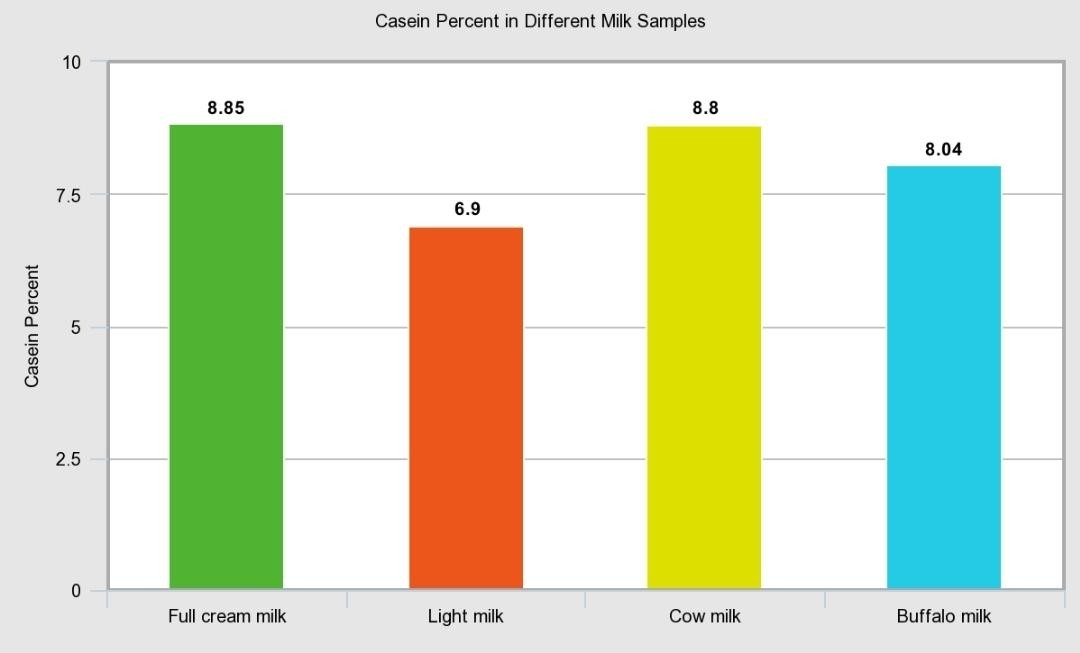
\includegraphics[width=0.5\textwidth]{bargraph.jpg}
    \caption{Bar graph of Casein Present in Different Milk Samples}
    \label{fig:my_figure}
\end{figure}

\section*{Acknowledgements}

The author wishes to acknowledge Mr. Sudeep Khanal for his suggestions on writing the article. 




\section*{References}

\begin{enumerate}
    \item Pioneer Chemistry Grade XII, First Edition, Dreamland Publication Pvt Ltd, Anamnagar, Kathmandu, Nepal  \vspace{-0.2cm}
    \item  Pioneer Practical Chemistry Grade XII, First Edition, Dreamland Publication Pvt Ltd, Anamnagar, Kathmandu, Nepal  \vspace{-0.2cm}
\end{enumerate}

\end{document}